\section{Contexto histórico}

La tulipomanía es probablemente la primera burbuja económica de la historia de la que existe información detallada y que ha sido estudiada en profundidad por economistas e historiadores. Tuvo lugar en Holanda, en el período que abarca del año 1.630 al 1.637.

Se ha de situar a Holanda en un contexto de auge económico y de desarrollo. Pocos años atrás, Holanda se había declarado independiente del Imperio español. De este modo, para instaurar su propia autonomía comercial internacional, tuvo que desarrollar su propia flota naval, aprender a tripularla y desplegarla. A la cabeza de esta iniciativa se encontraba la Compañía de las Indias Orientales, empresa cuya propiedad se dividía entre el gobierno y el sector privado. Esta empresa navegaba alrededor del mundo y se encargaba de obtener productos poco comunes en Europa para venderlos y obtener amplios beneficios. Con las provincias holandesas convertidas en el principal centro de comercio del norte de Europa, se alcanzó la llamada edad de oro holandesa.

El marco cronológico de la tulipomanía, es la Europa del siglo XVII. Al igual que en la actualidad, las clases sociales altas atribuían gran valor a aquellos objetos indicadores del elevado estatus social al que pertenecían. En el siglo XVII, estos objetos eran mansiones, jardines, e incluso ciertas flores exóticas, como el tulipán.

\section{El tulipán}

La primera referencia que existe sobre el tulipán, data de hace más de mil años y se establece su procedencia en Anatolia, región que se corresponde a la actual Turquía. 

\emph{Lale} es la traducción al turco y contiene las mismas letras que el Dios islámico \emph{Alá}, por lo que era considerada una flor sagrada. El tulipán, debido a su sencillez y belleza, encandiló a los altos representantes del Imperio Otomano.

Es conveniente, explicar previamente determinados aspectos relacionados con el desarrollo biológico del tulipán para la compresión del comportamiento del mercado de tulipanes que se llevó a cabo en Holanda.

En particular, se describirán brevemente los tiempos de desarrollo de un bulbo de tulipán, el florecimiento de dicho bulbo, la aparición de vástagos y la asombrosa aparición de tulipanes policromáticos, comúnmente denominados en inglés \emph{tulip flames}. 

\begin{figure}[!h] 
\caption{Semper Augusta} 
\centering 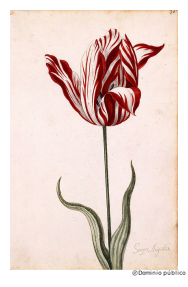
\includegraphics[width=50mm]{capitulos/img/semperAugustus} 
\label{fig:semperAugustus} 
\end{figure}

Los tulipanes son cultivados a partir de semillas. Éstas podrían tardar de tres a cinco años en convertirse en bulbo y de cinco a diez años en producir una flor. Cada bulbo, tiene el aspecto de una pequeña cebolla y puede llegar a producir al año uno o dos vástagos además de varias semillas. Un vástago es un pequeño bulbo que surge en la tierra a partir del bulbo matriz.

Tradicionalmente, la compra-venta de bulbos de tulipán se producía a lo largo de los meses de verano, cuando la flor nacida del bulbo, ya había florecido por el mes de mayo o junio (dependiendo de la clase de tulipán que se tratase). A continuación, la flor era cortada y vendida, y el bulbo se desenterraba, se envolvía en papel y se mantenía en lugares secos para su posterior inspección y replantación en el mes de septiembre.

Los tulipanes más codiciados por la sociedad en el siglo XVII, fueron los que tenían un único color como el rojo y el púrpura. Además, en 1.620 comenzaron a surgir tulipanes con extrañas y llamativas estructuras cromáticas o comúnmente denominados \emph{tulipanes con llamas}. Estas llamas, recorren simétricamente el centro de los pétalos y los bordes tal y como se puede apreciar en la Figura \ref{fig:semperAugustus}. Esta viva coloración que fascinó a los holandeses, fue causada por un virus que infecta los bulbos. Este hecho, fue un misterio en su momento ya que no se le dio explicación hasta el año 1.928, gracias a los trabajos de la doctora Dorothy Cayley. Este proceso impredecible añadió encanto y valor a los tulipanes como se comprobará a lo largo del capítulo.

\section{Origen y evolución del mercado de los tulipanes en Holanda}

La aparición del tulipán en Holanda fue posible gracias a dos personas fundamentalmente, Busbeq y Clusius.

En primer lugar, Ogier Ghiselin de Busbecq que fue un diplomático, escritor y herborista flamenco del siglo XVII, más conocido como \emph{Busbeq}.

Fue nombrado por Fernando I de Habsburgo como embajador del Sacro Imperio Romano Germánico en la corte de Solimán I el Magnífico. Fue enviado a Constantinopla a finales de 1.554 donde permaneció hasta 1.562. Durante esos años escribió las \emph{Cartas Turcas}, en las que relata sus experiencias y viajes en tierras del Imperio Otomano. En esta obra, a menudo resaltaba la hermosura de los jardines otomanos, con sus misteriosas flores rojas de tulipán. A su regreso a Austria, decidió llevar consigo algunos bulbos de esta planta. 

Busbeq entabló amistad con \emph{Carolus Clusius}, segundo hombre importante en la historia de la aparición del tulipán en Holanda. Se trató de un humanista, médico y botánico holandés, quien en 1.573 fue invitado por el emperador Maximiliano II de Habsburgo para trabajar para el jardín botánico de Viena. En ese lugar, Clusius plantó los bulbos de tulipán que con anterioridad Busbeq le confirió. Cuatro años más tarde, Clusius fue despedido y a lo largo de veinte años, se dedicó a viajar por toda Europa en busca de nuevos ejemplares.

En el otoño de 1.593, fue nombrado profesor honorario de botánica en la Universidad de Leiden, donde supervisó la creación de un jardín botánico. Entre la multitud de plantas del jardín, se encontraba su propia colección de bulbos de tulipán. En la primavera siguiente, es decir, en 1.594, surgieron los primeros tulipanes florecidos en el norte de Holanda. Una noche en la que Clusius se encontraba de viaje en Inglaterra, desenterraron su colección y la robaron.

Estos ladrones, de los que se desconoce su identidad, convirtieron a estos bulbos en los progenitores de las flores que más tarde inundarían los Países Bajos. A partir de este momento, comenzó el comercio del tulipán.

La ciudad holandesa de Haarlem, fue una de las primeras en llevar a cabo transacciones con tulipanes. El rápido enriquecimiento de una parte de la población hizo que otras ciudades, como Rotterdam o Leiden, tomasen ejemplo de ello, extendiéndose así el mercado de norte a sur y de este a oeste del país. Esta extensión del cultivo del tulipán y su comercio asociado, fue uno de los desencadenantes de la Edad de Oro holandesa.

Hasta principios de los años 30 del siglo XVII, el mercado de los tulipanes estaba compuesto por hombres sensatos de negocios, comerciantes ricos, cuyas fortunas no se verían afectadas por un fallido negocio de compra-venta de bulbos. También los herboristas, que poseían un amplio conocimiento de tan codiciada flor, eran partícipes en las transacciones. Pero el mercado alcanzó tal fama que las clases sociales medias y bajas también se introdujeron en él, realizando inversiones modestas y provocando un boom de inversiones. La mayoría de estos inversores de clase social media utilizaban los bulbos para la especulación. A pesar del gran número de variedades de tulipán, la oferta seguía siendo muy limitada y la demanda muy elevada.

\subsection{Tipos de contratos}

Para poder comprender el funcionamiento del mercado de tulipanes a partir de 1.634, se han de explicar los diferentes tipos de contratos que se dieron.

En primer lugar, los contratos de futuros. Garber (2.000) argumenta que, el comercio llevado a cabo en las tabernas, era un mercado plenamente de futuros: \emph{En la fecha de liquidación del contrato, se espera sólo el pago de la diferencia entre el contrato y el precio de liquidación. Este mercado no fue tan diferente a los mercados de futuros que operan actualmente}.

En segundo lugar, los contratos a plazos. Según informaciones que se han podido recopilar de contratos notariales y contratos menos formales de compra-venta de la época, parece ser que al menos algunas operaciones consistieron en una complicada cadena de contratos bilaterales a plazo que unen a varios vendedores y compradores. No existía ningún mecanismo de compensación central, pero en ocasiones los nuevos compradores acordaron asumir la deuda presente del vendedor, es decir, \emph{cuando mi comprador me pague, yo te lo pagaré}.

Y por último, los contratos al contado. Cabe destacar en este tipo de contratos, que los bulbos de tulipán no necesitan ser plantados en el campo con unas condiciones determinadas, sino que los tulipanes también crecen en macetas. Los individuos participantes en el mercado, regularmente tenían medios financieros para obtener vasijas hechas especialmente para el cultivo de la planta. De este modo, los tulipanes en macetas estarían disponibles para la venta y entrega inmediata. En segundo lugar, el desenterramiento de los tulipanes o en su defecto el transporte de estos, es posible pero no se recomienda, porque siempre existe un riesgo de dañar la planta. La opción de contratos con entrega inmediata, incluso en el período comprendido entre los meses de septiembre y de mayo-junio, es factible hasta el día 5 de febrero 1.637, última subasta de tulipanes con precios elevados.

\subsection{Las tabernas}

A continuación se explicará el mercado de tulipanes en las tabernas holandesas. En estos lugares se gestaba el comercio con un mayor grado de especulación. A los grupos sociales, tanto de taberneros como de clientes, se les denominó \emph{colleges}.

Haciendo una analogía para comprender el concepto de \emph{colleges}, se puede asemejar a las hermandades. Estas \emph{hermandades} estaban formadas por un núcleo de comerciantes regulares que se reunían dos o tres veces por semana y por lo general a la caída del día. Para pertenecer a este grupo, el individuo interesado debía de afiliarse a la compañía de los floristas, que poseían su sede en las diferentes tabernas de las ciudades. Así, cada miembro poseía una placa, a modo de código, con la que podía mercadear con los tulipanes a su antojo. Estas hermandades suponían un sistema muy intenso de redes sociales ya que aunque había que pertenecer a los colleges. Aún así, la accesibilidad era muy rápida y sencilla.

Este mercado se volvió mucho más arriesgado en el momento en el que se fueron incorporando individuos que no tenían ningún tipo de conocimiento acerca del funcionamiento del mercado. De este modo, el mercado se fue transformando poco a poco en una suerte de juego de azar en donde se podía doblar la cantidad jugada, y pagar así la deuda por el bulbo, o por el contrario, perder el bulbo y adquirir una mayor deuda alcanzando la completa ruina.

La mayor parte de la información recopilada acerca de las transacciones entre 1.636 y 1.637 de la que se dispone en la actualidad, es de una serie de contratos de tulipán individuales. Por lo general, estos documentos formaban parte del arbitraje a través de los notarios y de los tribunales. No se ha podido obtener información sobre la importancia relativa de las sesiones de negociación en las tabernas ya que no se dieron detalles sobre el tipo de transacciones, precios o volúmenes de comercio. Este tipo de negocio, era conocido en Holanda como \emph{Wind handle}, es decir, el negocio del aire.

Surgieron dos métodos de compra-venta de bulbos:

El primero, consistió en que tanto el comprador como el vendedor escribían un precio en un libro y elegían a una serie de mediadores que eran los encargados de fijar un precio intermedio, y mediante el arte del regateo conseguían cerrar el acuerdo. Este procedimiento se ejercía bien con contratos inmediatos o con contratos futuros.

El segundo método era la subasta. Se daba un precio de salida para una determinada transacción de bulbo, bulbos, tulipán o tulipanes, y se va incrementando este precio de salida hasta que ningún individuo está dispuesto a superar la oferta final.

En ambos casos, la gran mayoría de los negocios entre compradores y vendedores se llevaban a cabo con la presencia de los mediadores entendidos del mercado y que poseían amplios conocimientos acerca de los tulipanes.

Todos los contratos llevaban un suplemento de comida, bebida y tabaco llamado  \emph{Wijnkoop}, cuya traducción al castellano es  \emph{compra de vino}. Este coste era soportado por el comprador final y aproximadamente se correspondía con el 2,5 por ciento de la cantidad final pactada. Por otro lado, en el caso de la venta de futuros, si el bulbo desenterrado no se correspondía con las características pactadas meses antes, la venta quedaba anulada. En el caso de que se hubiese acordado un sistema de garantías, el avalista del comprador, bien sea amigo o pariente, garantizaría la devolución del pago y por lo tanto el vendedor podía atenerse a él.

A lo largo de la temporada de siembra del año 1.635, momento en el que los precios comenzaron a incrementarse, se produjo un cambio fundamental en la forma de comercialización de los bulbos en Holanda. Cada vez más a menudo, se vendían bulbos a peso mientras que éstos todavía se encontraban plantados en el campo. Tan sólo un \emph{pagaré}, indicaba los detalles del bulbo, incluyendo su peso en la siembra y el momento en el que se iba a proceder a desenterrarlo.

El peso de los bulbos se comenzó a medir en Azen o ass, una unidad de medida extremadamente pequeña que equivalía aproximadamente a una vigésima parte de un gramo, es decir, 0,05 gramos. Pagar en peso, era una manera más justa para evaluar el precio, ya que un bulbo inmaduro costaba menos que uno más maduro. La utilización de esta unidad de medida provocó el aumento del precio de los bulbos más pesados. Un bulbo que se planta en septiembre u octubre es probablemente mucho más pesado que en el momento en el que se desentierra, debido a que ha sufrido una floración. Lo que alentaba a la especulación en los siguientes meses estivales. Se puede afirmar, que el precio de los bulbos podría haber aumentado de un tres a un cinco por ciento en el transcurso de estos nueve meses, dependiendo del peso.

Esta nueva unidad de medida fue muy expandida y se comenzaron a vender grandes cantidades de bulbos a peso, es decir, surgió una nueva modalidad de transacciones, los contratos a granel. Lo que provocó que los precios aumentasen de nuevo poco a poco pero muy constantemente. Estos contratos al peso, tienen el mismo funcionamiento que los contratos de bulbos pero de una forma mucho más masificada, ya que se compran y venden grandes sumas de bulbos por cantidades enormes de florines.

\subsection{Estallido de la burbuja}

Con el desarrollo de los diferentes contratos explicados anteriormente y su progreso en las tabernas, además de la creación de la nueva unidad de medida, con la que surgieron los contratos a granel, el mercado fue adquiriendo consistencia y fue evolucionando de una forma mucho más rápida de lo que lo hacía cualquier otro mercado y por lo tanto aumentaba el propio poder adquisitivo de la población.

La burbuja especulativa no tardó en estallar. Los precios se incrementaron más rápidamente a partir de octubre de 1.636 y los contratos a granel fueron los más utilizados en diciembre de ese mismo año, otorgando al mercado un impulso final. A finales del 36, personas ajenas al mercado, predijeron una caída de precios inminente y en enero de 1.637 los precios aumentaron más rápido y los comerciantes sospechaban que la situación comenzaba a ser insostenible. Por otra parte, las redes sociales densas por parte de los colleges en las tabernas, provocaron que este conocimiento fuese común para todos los comerciantes.

El tres de febrero de 1.637, en la ciudad de Haarlem, se produjo el primer descenso de precios de una forma totalmente inesperada. El cinco de febrero del mismo año, en la ciudad de Alkmaar, el precio del tulipán consiguió su máximo histórico con la subasta, por parte de un orfanato que tutelaba a los siete hijos de un coleccionista fallecido. Éste poseía una serie de tulipanes de una rareza extrema. La subasta se llevó a cabo para salvaguardar la manutención de los sucesores y muchos holandeses se agolparon a las puertas del orfanato para poder participar en la mencionada subasta. Los 99 bulbos de tulipán fueron vendidos por 90.000 florines, es decir, era un contrato a granel ya que si se equipara tal cantidad de florines a los actuales euros, equivaldría aproximadamente a 7,6 millones de euros. El siete de febrero, el negocio se derrumbaba en los principales puntos de comercio holandeses.

De este modo, se puede asegurar que la burbuja estalló el ocho de febrero de 1.637, ya que ante nuevas subastas de tulipanes, no hubo compradores.


\subsection{Sátiras y fuentes de recopilación de datos sobre los precios de los tulipanes}

Con todo lo acontecido en la tulipomanía, no tardaron en aparecer numerosos folletos y obras de arte satíricas, donde se ridiculiza la exuberancia irracional de muchos participantes en el mercado de los tulipanes, como se puede apreciar en la Figura \ref{fig:Satire Of Tulip Mania} .


\begin{figure}[!h] 
	\caption{Fragmento de \emph{Satire Of Tulip Mania}, por Brueghel} 
	\centering
	\includegraphics[width=80mm]{capitulos/img/fragmentoSatireOfTulipMania-Brueghel} 
	\label{fig:Satire Of Tulip Mania} 
\end{figure}

Se pueden destacar los folletos publicados por Adriaen Roman en la ciudad holandesa de Haarlem. En estos folletos se mantiene un diálogo entre dos personajes principales, \emph{Gaergoedt}, y \emph{Waermondt}.

Gaergoedt interpreta un papel de comerciante activo y responsable de bulbos, que se compromete a educar a Waermondt en el mercado del tulipán con el fin de explicar y defender las acciones emprendidas por los consumidores. Por otro lado, Waermondt, relata cuentos moralistas con los que se pretende resaltar la insensatez en diversos aspectos de la tulipomanía. Una de las características más valiosas de estos diálogos es que se reproducen contratos reales de ventas de bulbos y da referencias aproximadas de los precios alcanzados por los bulbos de principio a fin del fenómeno.

No existe una sola fuente completamente fiable en cuanto a precios de los tulipanes se refiere. Existen alrededor de cuatrocientos precios diferentes y la gran mayoría de ellos hacen referencia a los máximos alcanzados por las diferentes clases de tulipanes.

Para superar esta ausencia de información, algunos autores han adoptado diferentes estrategias, como por ejemplo, confiar en los folletos publicados y escritos entre febrero y mayo de 1.637 por Adriaen Roman.

Por ejemplo, en el primer diálogo entre Gaergoedt y Waermondt, se afirma que \emph{algunos precios de bulbos despuntaron hasta tal punto que alcanzaron cifras desorbitadas}. Hay que recordar que estos diálogos están destinados a ilustrar el carácter dramático de este escandaloso aumento de precios.

Un enfoque más prometedor, es el que realiza Garber (2.000), quien genera dieciséis gráficos que muestran la evolución de los precios de las diferentes variedades de tulipanes. Estos gráficos demuestran que los precios aumentaron considerablemente, aunque no se pueden obtener conclusiones certeras acerca de la trayectoria de los precios. El método empleado, establece un patrón con una línea recta entre diferentes precios. Los precios utilizados pertenecen a diferentes fuentes de información, por lo que en ocasiones se emplea una media y en otras ocasiones accede a fiarse de un dato terminado.

Como se podrá comprobar a continuación, se puede apreciar un aumento gradual en la primera fase de la tulipomanía y más tarde, se da una pendiente mucho más empinada próxima al final de la burbuja. Como también existe escasez de datos tras el estallido de la burbuja, Garber se ve obligado a depender de los precios de venta entre 1.642 y 1.643 realizando de este modo una media anual. Sin embargo, Garber concluye que, \emph{la crisis en febrero de 1.637, en cuanto a los tulipanes se refiere, no fue de extraordinaria magnitud} y la asume simplemente como una caída de precios gradual para el período comprendido entre 1.637 y 1.642. Garber considera que esta caída entra dentro de la normalidad del funcionamiento del mercado, es decir, Garber razona que la tulipomanía no es una burbuja económica como tal.

En las páginas posteriores se reflejan los gráficos de precios de algunos de los tulipanes más destacados a lo largo del desarrollo de la tulipomanía según las estimaciones de Peter Garber. Se corresponden a las figuras \ref{fig:Semper Augusta}, \ref{fig:Admirante Van Der Eyck}, \ref{fig:Admirante Liefkens} y \ref{fig:Switsers}


\begin{figure}[!h] 
\caption{Semper Augusta} 
\centering \includegraphics[width=150mm]{capitulos/graficos/SemperAugusta} 
\label{fig:Semper Augusta} 
	\footnotesize
	Fuente: Estimaciones de Peter Garber (2.000)
\end{figure}

\begin{figure}[!h] 
\caption{Admirante Van der Eyck} 
\centering \includegraphics[width=150mm]{capitulos/graficos/AdmiranteVanDerEyck} 
\label{fig:Admirante Van Der Eyck} 
	\footnotesize
	Fuente: Estimaciones de Peter Garber (2.000)
\end{figure}

\begin{figure}[!h] 
\caption{Admirante Liefkens} 
\centering 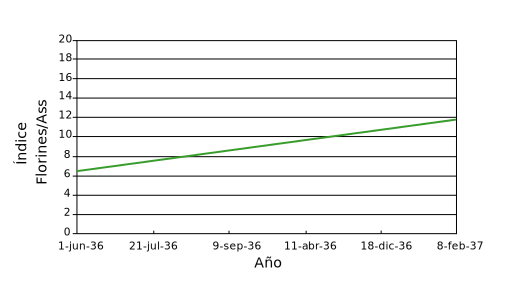
\includegraphics[width=150mm]{capitulos/graficos/AdmiranteLiefkens} 
\label{fig:Admirante Liefkens} 
	\footnotesize
	Fuente: Estimaciones de Peter Garber (2.000)
\end{figure}

\begin{figure}[!h] 
\caption{Switsers} 
\centering \includegraphics[width=150mm]{capitulos/graficos/Switsers} 
\label{fig:Switsers} 
	\footnotesize
	Fuente: Estimaciones de Peter Garber (2.000)
\end{figure}


En cuanto al momento del colapso, el primer lugar donde se produjo un descenso de precios fue en la ciudad de Haarlem el 3 de febrero. En los escritos de Adrien Roman, el protagonista Waermondt, narra el episodio donde los miembros de una hermandad decidieron poner a prueba la confianza del mercado, poniendo a la venta gran cantidad de tulipanes comunes como lo eran \emph{Switsers o Croonen} donde sólo se dio un comprador y éste mismo comprador ofreció diferentes precios en las tres subastas donde los tres vendedores aceptaron su oferta, a pesar de que la suma que ofreció fue una sucesión a la baja, comenzando en un 15 por ciento por debajo del precio de ese momento, continuando en un 25 por ciento y finalmente llegando al 35 por ciento. La noticia de esta caída en picado de los precios se extendió por todo el pueblo, pero no por el resto de Holanda. Dos días más tarde, en una subasta en Alkmaar, se alcanzaron los precios máximos.

Las notas de Gaergoedt ratifican la dificultad de establecer un nivel de precios tras el estallido de la burbuja y lo expresa en esta frase: \emph{Desde que no existe demanda, todo el mundo permanece en silencio}. Estima que tras el estallido, un jardín con tulipanes comunes no tenía ni la centésima parte del valor de hace tan solo unas semanas. Esto se puede comprobar con un claro ejemplo, un bulbo que valió en noviembre de 1.636 cuatrocientos florines, tras el estallido de la burbuja su precio descendió a veintidós florines, lo que supondría desmentir la tesis de Garber de caída de precios constante. 

Las fuentes de información son un aspecto clave para la realización de un exhaustivo estudio de precios. El fallecido profesor de la Universidad de Stanford, Earl. A. Thompson (2006), en su estudio \emph{The Tulipmania: Fact or Artifact}, ratificó que el aumento de los precios de los tulipanes a principios de 1.637 se debió a una serie de cambios en los instrumentos del mercado de los contratos futuros. Este autor, basa sus estudios en la validez de un índice generado por él mismo a través de precios relativos constantes, y que permite comparar diferentes tipos de tulipanes. Como punto negativo, se ha de señalar que no tiene en cuenta dos aspectos fundamentales como son, el espacio temporal, ya que no emplea el mismo momento temporal para todos ellos; y que evalúa al mismo tiempo los diferentes contratos\footnote{Los contratos con los vástagos de los bulbos, con los propios bulbos y con los bulbos vendidos a granel.} sin tener en cuenta que el valor de las transacciones no es igual para cada uno de ellos. A continuación se muestra la Figura \ref{fig:Precios de la tulipomanía según Thompson} donde se puede observar gráficamente su estudio:

\begin{figure}[!h] 
\caption{Precios de la tulipomanía según Thompson} 
\centering 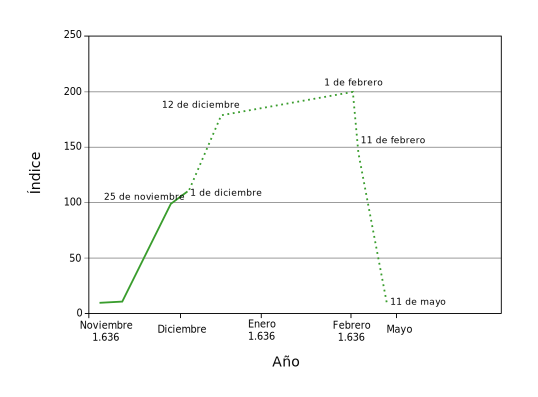
\includegraphics[width=150mm]{capitulos/graficos/Thompson} 
\label{fig:Precios de la tulipomanía según Thompson} 
	\footnotesize
	Fuente:  Earl A. Thompson (2.007)
\end{figure}

Thompson concluye que la centenaria literatura ha tergiversado la verdadera historia de la Tulipomanía. Pero por el contrario, da credibilidad a una serie de precios de los tulipanes de antes, durante y después de Tulipomanía, ya que afirma que proporcionan una información notable de los precios de mercado eficiente. Defiende que en su gráfico, los precios se pueden observar con rapidez y precisión, y se refleja la economía subyacente de un mercado en el que la euforia se traduce en ganancias y la decepción en pérdidas de capital.

En resumen, los datos de Garber y de Thompson no son de todo fiables. Las fluctuaciones de precios no son apoyadas por los fundamentos del mercado, ya que por ejemplo Garber ignora los puntos clave descritos en el párrafo anterior. Realizar afirmaciones más precisas sobre el precio, como por ejemplo cuándo y cómo se produjeron ciertos hechos en la burbuja económica es muy complicado. Por otro lado, Thompson ignora los problemas de la agregación de información de precios en los diferentes momentos temporales, aplicados a las diferentes formas de compra-venta de bulbos. Pese a que los datos son limitados, indican un rápido aumento entre diciembre de 1.636 y enero 1.637, seguido de un descenso brutal.

Para finalizar este epígrafe, hay que desatacar que por ejemplo Garber, establece una aproximación más bien gráfica, ya que realizar afirmaciones más precisas sobre cuándo y cómo se produjeron ciertos hechos en esta burbuja es muy complicado. En cuanto a Thompson, éste ignora los problemas de escasez de datos anteriormente descritos. Como conclusión al estudio de precios, se puede afirmar que los datos de Garber y de Thompson no son cien por cien fiables debido a la escasez de información que la tulipomanía sufre. 


\subsection{Influencia de la redes sociales} 

Para alcanzar una mayor comprensión de cómo se fueron desencadenando los hechos en la tulipomanía, se debe tener en cuenta un factor moderno como son las redes sociales, pero que inconscientemente ya era patente en el siglo XVII.

En primer lugar, se debería destacar la audacia de los vendedores, cada vez más experimentados, que se percataron de que cuanta más gente conociese su producto, más aumentarían las ventas y los precios de éstos, por lo que se creó el primer catálogo floral de ventas titulado \emph{El catálogo floral}, cuyo autor fue Emanuel Sweertl, también comerciante de tulipanes. Dicho libro, con pobres ilustraciones de los tulipanes en venta, hizo que se exportase en mayor medida tan codiciada flor. A raíz de este descubrimiento publicitario, se escribieron otros muchos que consiguieron ser número uno de ventas y provocaron, como bien había predicho Sweertl, el incremento del precio de los tulipanes.

Pese a la existencia de los catálogos florales, se puede percibir la ausencia de uno de los elementos más importantes y que hoy en día es imprescindible, los medios de comunicación. La importancia de éstos proviene de ser una de las necesidades primarias del ser humano: \emph{la interacción social}. Además, en la actualidad influye la \emph{opinión pública}. Como ejemplo, la influencia que tuvieron los medios de comunicación al mando de   Hitler como táctica para manipular a la sociedad alemana para que apoyara su ideología. Retomando la tulipomanía, es destacable la ausencia de periódicos regulares para cubrir la evolución del mercado de los tulipanes, el colapso de los precios y la consecuente crisis. Los periódicos, surgieron en las ciudades más desarrolladas de Holanda en el año 1.660, tres décadas después de la tulipomanía.

Otro de los aspectos a tener en cuenta, en el desarrollo de esta burbuja, es la eficacia de las redes sociales y las intensas normas de convivencia que la rodean.

Los comerciantes de tulipanes solían estar ligados entre si de una forma personal, bien por lazos familiares, por pertenecer al mismo grupo religioso o por compartir lugares de trabajo. Este hecho permitía que los integrantes del mercado permaneciesen influenciados por el propio mercado ya que daban una excesiva credibilidad a las decisiones de otros compradores y vendedores conocidos entre sí. Este fenómeno lleva a Shiller (2.000) a defender la hipótesis de que la burbuja fue el resultado de una \emph{cascada de información}. La idea básica asociada a este término es ignorar el conocimiento propio y seguir las decisiones de los demás integrantes del mercado. Este comportamiento, está relacionado con lo que en economía conductual (behavioral economics) se conoce como \emph{herding} o \emph{comportamiento de manada}. Se recuerda que este es un término  que trata de definir un comportamiento en el que personas influyentes en el mercado, convencen a los compradores potenciales menos experimentados, para seguir el comportamiento masificado de compra ya sea correcto o incorrecto. De este modo, se sigue a uno o varios líderes que consiguen que el \emph{rebaño} siga sus movimientos a ciegas. No es difícil imaginarlo en un contexto social en el que los agentes confían unos en otros y viceversa. En el caso de los tulipanes, el efecto de comportamiento de manada se puede apreciar claramente ya que los precios comenzaron a subir alimentados por los compradores que casi siempre optaban por los mismos bulbos impulsados por la moda. De este modo, la demanda de unos determinados bulbos se disparó pese a que la oferta continuaba siendo escasa.

Se podría plantear una pregunta importante para la correcta explicación del funcionamiento del mercado de los tulipanes, \emph{¿Qué estrategias adoptaban los compradores de tulipanes?} Por ejemplo, si un comprador de tulipanes en el siglo XVII permanece en el mercado el suficiente tiempo como para haber llevado a cabo compras y ventas con la planta durante años, conocerá a la mayoría de los agentes del comercio y confiará en los conocimientos y juicios de los que sean expertos. Si este comprador busca una clase determinada de tulipán puede adoptar tres estrategias:

\begin{enumerate}
	\item Investigar la evolución del mercado del tulipán para empaparse de información y poder determinar un valor razonable.
	\item Comprobar si algún comprador ha participado en subastas de bulbos con características semejantes y qué clase de ofertas llega a tramitar.
	\item Superar la oferta de un comerciante conocido y fiable, pero abandonar el mercado si existe una oferta mayor de otro agente desconocido para no asumir riesgos.
\end{enumerate}

De esta forma y atraídos por el dinero fácil o por haber adquirido una importante inyección de liquidez, se introducen en el mercado un conjunto de novatos: de $X_1$ a $X_n$. Estos nuevos integrantes deciden comenzar a comprar tulipanes. Debido a su desconocimiento del mercado, en un primer momento podrían adoptar las estrategias dos y tres, es decir, informarse de los precios de una forma contrastada, bien por el mercado o bien por amistades fiables. Este hecho reduciría la fracción de los participantes en la subasta con conocimiento privilegiado y como resultado, existiría una probabilidad más pequeña de que cada comprador y vendedor obtuviese información valiosa, por lo que, algunos novatos podrían empezar a confiar en otros novatos, pensando que en realidad, son expertos. 


Teniendo en cuenta los párrafos anteriores, se puede apreciar la necesidad de tener en cuenta, a la hora de realizar estudios, las variables como el suministro de bulbos, la naturaleza de los contratos de compra-venta de tulipanes y la comunidad de comerciantes de tulipán. 


A medida que la burbuja continuaba hinchándose, el suministro de bulbos se incrementaba a través del aumento de la producción de vástagos. Los productores que disponían de bulbos raros, que eran los más solicitados, se encontraban en una situación muy cómoda ya que mantenían el control prácticamente absoluto del mercado. La rápida expansión de comerciantes y de expertos en la materia en Holanda provocó que la demanda aumentase notablemente. A principios de 1.630, la demanda era más alta que la oferta, por lo que no era de extrañar que los precios aumentasen, o por el contrario, que se comenzasen a vender bulbos de peor calidad. Este crecimiento de los precios atrajo a más comerciantes.


Si se siguen las leyes de la economía, es de suponer que en una situación \emph{normal} de mercado, la economía se encuentra en equilibrio, pero en el caso de la tulipomanía, la demanda de un bulbo crecía más rápido de lo que lo hacía su oferta. También se puede recalcar que el poder adquisitivo por parte de los burgueses ricos crecía más pausadamente en comparación con los precios de los tulipanes. 


El mercado del tulipán funcionó eficientemente hasta que los comerciantes noveles se iniciaron en el mercado, entonces éste se hizo menos estable por la dificultad que entrañaba distinguir entre los individuos que poseían conocimientos privados sólidos y los que estaban simplemente siguiendo a la multitud.


En el momento previo al colapso, los comerciantes veteranos llevaron a cabo las estrategias dos y tres, es decir, comprobar si algún comprador había participado en subastas de bulbos con características semejantes y qué clase de ofertas se tramitaban. También puede optar por la posibilidad de superar la oferta de algún comprador conocido y fiable, pero abandonar el mercado si existe una oferta mayor de otro agente desconocido. La elección de estas estrategias provocaba un aumento de precios destacable.


En enero de 1.637, los precios aumentaron mucho más intensa y rápidamente y los comerciantes comenzaban a sospechar que la situación empezaba a ser insostenible. Por otra parte, las densas redes sociales provocaron que este conocimiento fuese común a todos los comerciantes.


Para concluir este largo camino de seis años en los que la tulipomanía tardó en alcanzar su punto álgido, se ha de establecer que dicho colapso se produjo, en gran medida, por el cambio de apreciación de los compradores hacia las flores, ya que el precio que estaban pagando hasta entonces era muy superior al valor fundamental de los bulbos y las flores. 

